\section{Results}
\label{sec:results}

We first report task scores across tiers (\secref{sec:res_scores}), then the primary \standard\versus\exhaustive contrast and its dependence on model size (\secref{sec:res_drop}), format compliance (\secref{sec:res_compliance}), and finally the padding and placement controls that test the mechanism (\secref{sec:res_padding}).
\Tabref{tab:verdicts} summarizes the verdict for each hypothesis.

\begin{figure}[t]
\centering
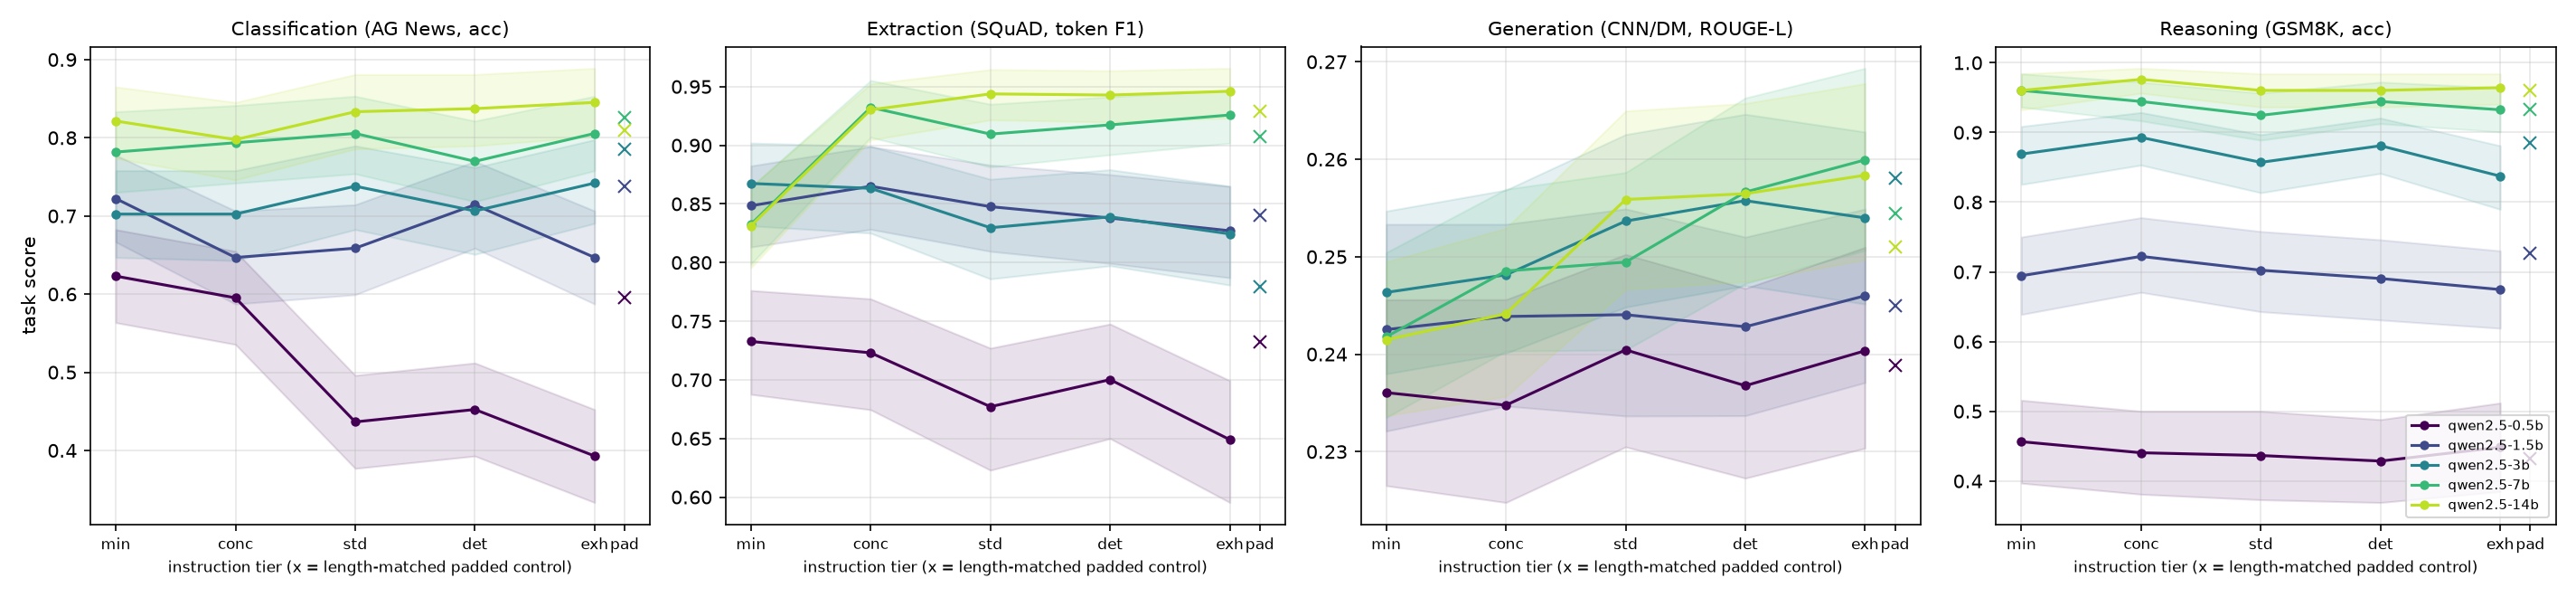
\includegraphics[width=\linewidth]{figures/score_by_tier.png}
\caption{Task score \versus instruction tier for five \qwen sizes. Shaded areas are 95\% bootstrap CIs; $\times$ marks the length-matched \padded control. For $\geq$3B models the curves are flat or slowly rising after \concise. The only steep decline is the 0.5B model on classification (and, more mildly, extraction), and the \padded control (same content as \standard, length of \exhaustive) sits near the \minimal level rather than the \exhaustive level.}
\label{fig:scores}
\end{figure}

\begin{table}[t]
\centering
\caption{Task score (\%) by instruction tier, $n=252$ items per cell. Classification and reasoning are accuracy, extraction is token F1, and generation is ROUGE-L F1. The best condition per row is in {\bf bold}. Binary-metric 95\% CIs are about $\pm$5--6 points; ROUGE-L CIs are about $\pm$1 point. For $\geq$3B models, \standard and \exhaustive are within 1.6 points on every task. Only the 0.5B model shows a large decline with length, and the \padded control does not reproduce it.}
\label{tab:main}
\small
\begin{tabular}{@{}llcccccc@{}}
\toprule
Task & Model & \minimal & \concise & \standard & \detailed & \exhaustive & \padded \\
\midrule
\multirow{5}{*}{\shortstack[l]{\textsc{Cls}\\(\agnews)}}
 & 0.5B & {\bf 62.3} & 59.5 & 43.7 & 45.2 & 39.3 & 59.5 \\
 & 1.5B & 72.2 & 64.7 & 65.9 & 71.4 & 64.7 & {\bf 73.8} \\
 & 3B   & 70.2 & 70.2 & 73.8 & 70.6 & 74.2 & {\bf 78.6} \\
 & 7B   & 78.2 & 79.4 & 80.6 & 77.0 & 80.6 & {\bf 82.5} \\
 & 14B  & 82.1 & 79.8 & 83.3 & 83.7 & {\bf 84.5} & 81.0 \\
\midrule
\multirow{5}{*}{\shortstack[l]{\textsc{Ext}\\(\squad)}}
 & 0.5B & {\bf 73.3} & 72.3 & 67.7 & 70.0 & 64.9 & 73.2 \\
 & 1.5B & 84.8 & {\bf 86.5} & 84.8 & 83.8 & 82.7 & 84.0 \\
 & 3B   & {\bf 86.7} & 86.3 & 83.0 & 83.9 & 82.4 & 77.9 \\
 & 7B   & 83.3 & {\bf 93.2} & 91.0 & 91.7 & 92.6 & 90.8 \\
 & 14B  & 83.1 & 93.0 & 94.4 & 94.3 & {\bf 94.6} & 92.9 \\
\midrule
\multirow{5}{*}{\shortstack[l]{\textsc{Gen}\\(\cnndm)}}
 & 0.5B & 23.6 & 23.5 & {\bf 24.0} & 23.7 & {\bf 24.0} & 23.9 \\
 & 1.5B & 24.3 & 24.4 & 24.4 & 24.3 & {\bf 24.6} & 24.5 \\
 & 3B   & 24.6 & 24.8 & 25.4 & 25.6 & 25.4 & {\bf 25.8} \\
 & 7B   & 24.2 & 24.9 & 24.9 & 25.7 & {\bf 26.0} & 25.4 \\
 & 14B  & 24.1 & 24.4 & 25.6 & 25.6 & {\bf 25.8} & 25.1 \\
\midrule
\multirow{5}{*}{\shortstack[l]{\textsc{Rsn}\\(\gsm)}}
 & 0.5B & {\bf 45.6} & 44.0 & 43.7 & 42.9 & 44.8 & 43.3 \\
 & 1.5B & 69.4 & 72.2 & 70.2 & 69.0 & 67.5 & {\bf 72.6} \\
 & 3B   & 86.9 & {\bf 89.3} & 85.7 & 88.1 & 83.7 & 88.5 \\
 & 7B   & {\bf 96.0} & 94.4 & 92.5 & 94.4 & 93.3 & 93.3 \\
 & 14B  & 96.0 & {\bf 97.6} & 96.0 & 96.0 & 96.4 & 96.0 \\
\bottomrule
\end{tabular}
\end{table}


\subsection{Task scores are flat across tiers for models of 3B and above}
\label{sec:res_scores}

\Figref{fig:scores} and \tabref{tab:main} show task scores for all conditions.
{\bf For 3B--14B models, the curves are flat after the first step.}
Classification accuracy for 7B stays between 77.0\% and 80.6\% across all five tiers, and 14B stays between 79.8\% and 84.5\%.
Reasoning accuracy for 14B ranges only from 96.0\% to 97.6\%.
Where we see a clear change, it comes from the shortest instruction.
For extraction, moving from \minimal to \concise raises 7B F1 from 83.3 to 93.2 and 14B F1 from 83.1 to 93.0.
The \minimal prompt makes models return spans that are too long: the 7B model's mean answer length is 5.0 words at \minimal and 3.1--3.3 words at every longer tier.
Once the instruction defines what a good span is, further detail neither helps nor hurts.

{\bf Generation improves slowly and does not plateau.}
ROUGE-L for $\geq$3B models rises from 24.1--24.6 at \minimal to 25.4--26.0 at \exhaustive.
The per-tier slope from \minimal to \detailed is $+0.34$ [0.10, 0.57] points for 3B, $+0.45$ [0.21, 0.69] for 7B, and $+0.57$ [0.32, 0.82] for 14B.
Every consecutive step is positive, but no single step is significant on its own.
The gain continues to \exhaustive rather than peaking at \detailed.
The 0.5B and 1.5B models show a slope of about zero.

{\bf The smallest model is the exception.}
For 0.5B, the \minimal tier is the best tier on three of four tasks.
Classification accuracy drops from 62.3\% at \minimal to 43.7\% at \standard and 39.3\% at \exhaustive, and extraction F1 drops from 73.3 to 64.9.

\subsection{The standard-to-exhaustive drop shrinks with model size, but 7B is not special}
\label{sec:res_drop}

\begin{table}[t]
\centering
\caption{Primary contrast: \standard $-$ \exhaustive, in points with 95\% bootstrap CIs. Positive values mean the \exhaustive tier hurts. Uncorrected permutation $p$-values are shown where $p<.1$. After Holm correction over these 20 tests, only 7B generation is significant ($p_{\text{holm}}=.02$), and there \exhaustive \emph{helps}. The 0.5B classification drop has $p_{\text{holm}}=.25$.}
\label{tab:drop}
\small
\begin{tabular}{@{}lcccc@{}}
\toprule
Model & \textsc{Cls} & \textsc{Ext} & \textsc{Gen} & \textsc{Rsn} \\
\midrule
0.5B & $+4.4$ {\scriptsize [1.2, 7.5]} $p{=}.013$ & $+2.8$ {\scriptsize [$-1.2$, 6.7]} & \phantom{$+$}$0.0$ {\scriptsize [$-0.7$, 0.7]} & $-1.2$ {\scriptsize [$-7.5$, 5.2]} \\
1.5B & $+1.2$ {\scriptsize [$-2.0$, 4.4]} & $+2.1$ {\scriptsize [$-0.7$, 4.9]} & $-0.2$ {\scriptsize [$-0.9$, 0.5]} & $+2.8$ {\scriptsize [$-2.8$, 8.3]} \\
3B   & $-0.4$ {\scriptsize [$-4.0$, 3.2]} & $+0.5$ {\scriptsize [$-2.5$, 3.5]} & \phantom{$+$}$0.0$ {\scriptsize [$-0.6$, 0.6]} & $+2.0$ {\scriptsize [$-2.0$, 6.3]} \\
7B   & \phantom{$+$}$0.0$ {\scriptsize [$-2.4$, 2.4]} & $-1.6$ {\scriptsize [$-3.5$, 0.0]} $p{=}.06$ & {\bf $-$1.0} {\scriptsize [$-1.7$, $-0.4$]} $p{=}.001$ & $-0.8$ {\scriptsize [$-4.4$, 2.8]} \\
14B  & $-1.2$ {\scriptsize [$-4.4$, 2.0]} & $-0.2$ {\scriptsize [$-1.3$, 0.8]} & $-0.2$ {\scriptsize [$-0.8$, 0.3]} & $-0.4$ {\scriptsize [$-2.4$, 1.6]} \\
\bottomrule
\end{tabular}
\end{table}


\begin{figure}[t]
\centering
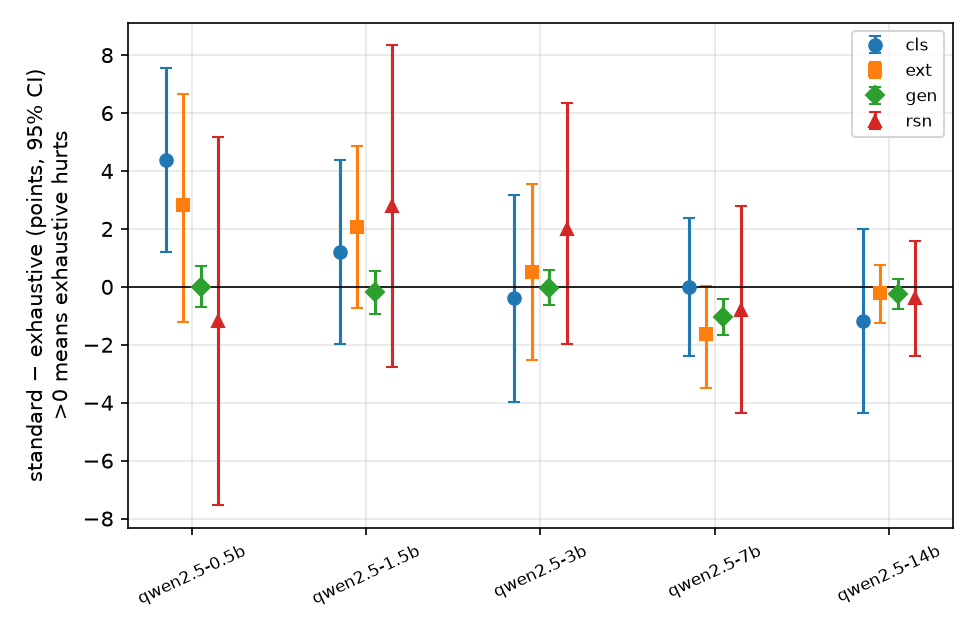
\includegraphics[width=0.6\linewidth]{figures/drop_by_model.png}
\caption{\standard $-$ \exhaustive difference per model and task, with 95\% bootstrap CIs. Values above zero mean the longer instruction hurts. Only the 0.5B classification interval lies fully above zero; for 7B and 14B all point estimates are at or below zero.}
\label{fig:drop}
\end{figure}

H1 predicts a 3--7 point drop from \standard to \exhaustive for classification and extraction.
\Tabref{tab:drop} and \figref{fig:drop} show that this drop does not appear for models of 1.5B and above.
For $\geq$1.5B, the drop is at most $+1.2$ points on classification and $+2.1$ on extraction, and no interval excludes zero in the predicted direction.
For 7B and 14B, all point estimates are zero or negative, so the longer instruction is, if anything, slightly better.
After Holm correction over the 20 primary tests, the only significant difference is 7B generation, where \exhaustive is 1.0 ROUGE-L point \emph{better} ($p_{\text{holm}}=.02$).
The 0.5B classification drop of 4.4 points is significant before correction ($p=.013$) but not after ($p_{\text{holm}}=.25$).

H4 predicts that 7B degrades more than larger models.
It does not: the 7B $-$ 14B difference-in-differences is $+1.2$ [$-3.2$, 5.6] for classification, $-1.4$ [$-3.4$, 0.5] for extraction, $-0.8$ for generation, and $-0.4$ for reasoning, all not significant.
A generalized form of H4 does hold.
Across the five sizes, the \standard$\to$\exhaustive drop decreases with log model size (Spearman $\rho=-0.9$, $p=.037$, for both classification and extraction).
With only five points this correlation is fragile, and the effect is concentrated below 2B parameters rather than spread across the range.

H3 predicts no change in reasoning beyond \concise.
Cochran's Q over \concise$\to$\exhaustive gives $p=.93$, .37, .056, .50, and .30 for the five sizes, so we find no significant differences.
However, we cannot establish equivalence within $\pm$3 points for most models, and 3B shows a 5.6-point dip from \concise to \exhaustive (90\% CI [$-9.5$, $-1.6$]).
The \exhaustive tier also changes \emph{how} models reason.
The 7B model follows the prescribed verification steps and produces outputs twice as long (437 \versus 214 tokens at \standard), with no change in accuracy.

\subsection{Format compliance saturates early}
\label{sec:res_compliance}

\begin{figure}[t]
\centering
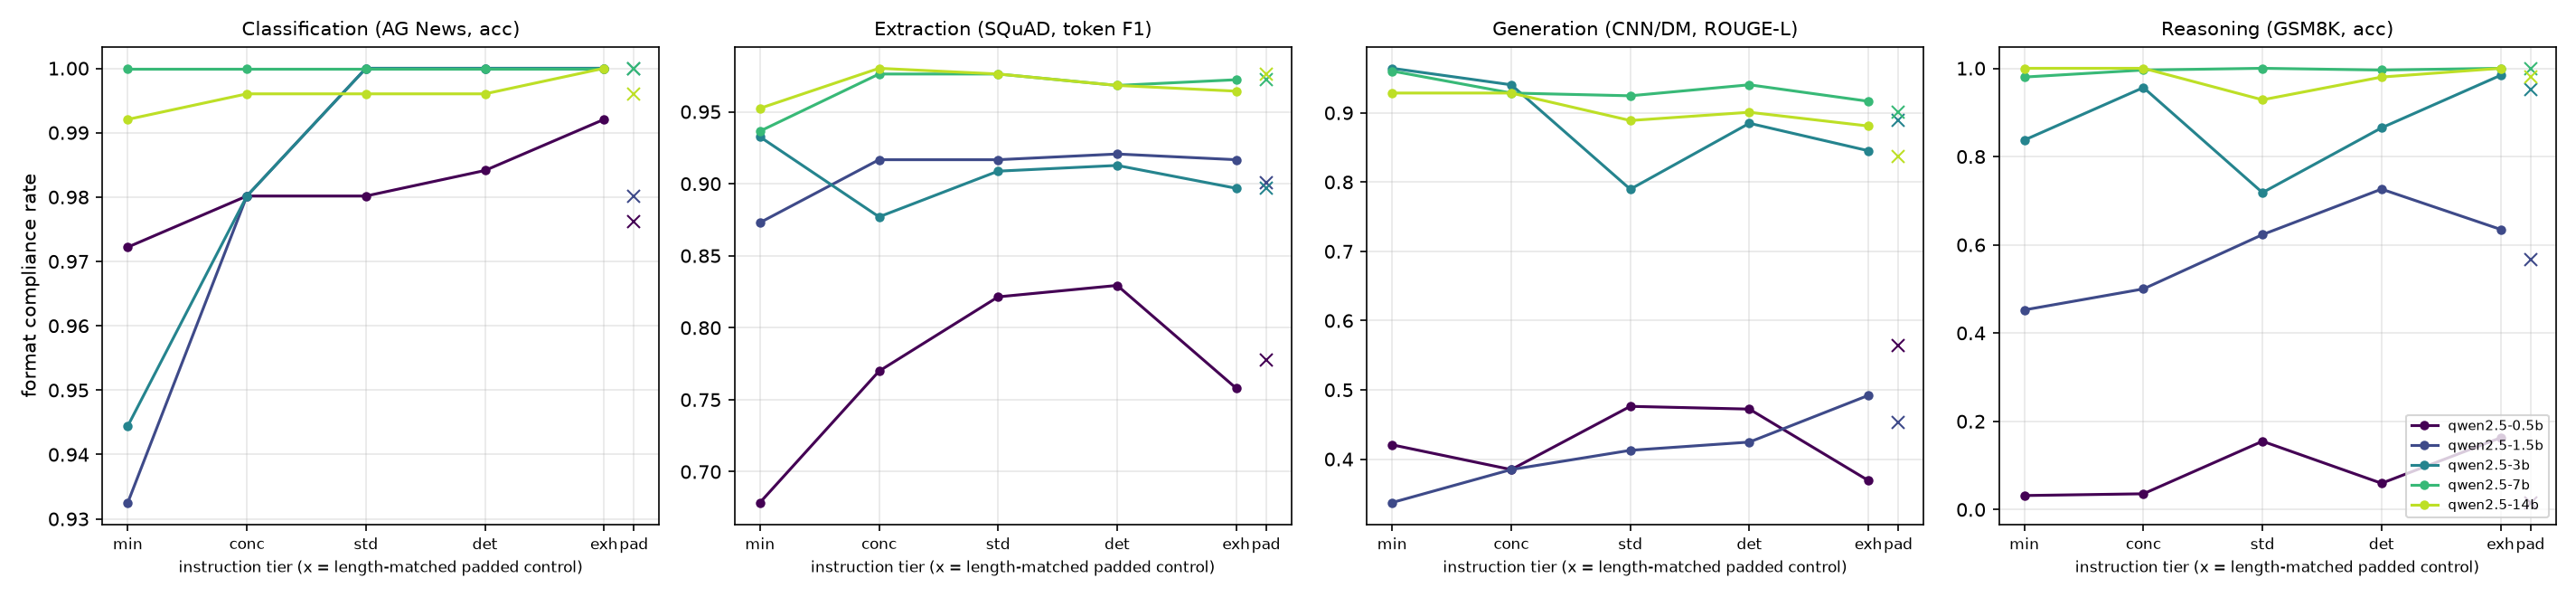
\includegraphics[width=\linewidth]{figures/compliance_by_tier.png}
\caption{Strict format-compliance rate \versus instruction tier (panel titles name the task; the y-axis is compliance, not task score). $\times$ marks the \padded control. Models of 7B and above reach 88--100\% compliance from \concise onward. The small models show no common peak, and for reasoning the \exhaustive tier, which ends by restating the format, is often the most compliant.}
\label{fig:compliance}
\end{figure}

H5 predicts that compliance peaks at \standard for every task.
\Figref{fig:compliance} shows that it does not.
\standard is the unique maximum in only 1 of 20 model$\times$task cells (0.5B generation), and is tied for the maximum in 5 more cells, all at or near 100\%.
The common pattern is a ceiling from \concise onward: $\geq$7B models comply 88--100\% of the time at every tier from \concise to \exhaustive.
For small models the peak tier is scattered.
Restating the format at the end of the prompt matters for reasoning: 3B compliance is 72\% at \standard and 98\% at \exhaustive.
Most reasoning violations are cosmetic, such as bold markdown (\texttt{**Final answer: 20**}) or LaTeX layouts.
The 0.5B and 1.5B models violate the generation constraint (2--4 sentences, $\leq$80 words) more than half the time at every tier.

\subsection{Length alone does not hurt: padding and placement controls}
\label{sec:res_padding}

\begin{table}[t]
\centering
\caption{Padding control. \padded has the content of \standard and the word count of \exhaustive. Differences are in points with 95\% bootstrap CIs; $p_{\text{holm}}$ is corrected over the 40 padding tests. Filler never significantly hurts after correction; for the small models it significantly \emph{helps} relative to \standard, while the content-rich \exhaustive tier is significantly worse than \padded.}
\label{tab:padding}
\resizebox{\textwidth}{!}{%
\begin{tabular}{@{}lccccc@{}}
\toprule
Model / task & \standard & \exhaustive & \padded & \padded $-$ \standard & \exhaustive $-$ \padded \\
\midrule
0.5B \textsc{Cls} & 43.7 & 39.3 & {\bf 59.5} & $+15.9$ {\scriptsize [11.1, 20.6]} \increase & $-20.2$ {\scriptsize [$-25.4$, $-15.1$]} \decrease \\
1.5B \textsc{Cls} & 65.9 & 64.7 & {\bf 73.8} & $+7.9$ {\scriptsize [4.4, 11.9]} \increase & $-9.1$ {\scriptsize [$-13.1$, $-5.2$]} \decrease \\
0.5B \textsc{Ext} & 67.7 & 64.9 & {\bf 73.2} & $+5.5$ {\scriptsize [0.9, 10.3]} & $-8.3$ {\scriptsize [$-12.9$, $-3.8$]} \decrease \\
\midrule
$\geq$3B, all tasks & \multicolumn{5}{c}{all differences within $\pm$5.1 points; none significant after correction} \\
\bottomrule
\end{tabular}%
}
\end{table}

H6 asks whether any harm from long instructions comes from token count or from content.
\Tabref{tab:padding} gives a clear answer: {\bf irrelevant filler of the same length does not reproduce the harm.}
For 0.5B classification, \padded reaches 59.5\%, 15.9 points above \standard and 20.2 points above \exhaustive ($p_{\text{holm}}=.008$ for both).
1.5B classification shows the same pattern ($+7.9$ and $-9.1$ points, $p_{\text{holm}}=.008$), and \exhaustive is 8.3 points below \padded for 0.5B extraction ($p_{\text{holm}}=.014$).
For $\geq$3B models, no padding difference survives correction.
The largest uncorrected effect is 3B extraction, where \padded is 5.1 points below \standard ($p=.005$ uncorrected), so filler is not entirely harmless; but across 40 tests it never significantly hurts after correction.
We therefore reject the pure token-dilution account in this length range.

\para{Instruction placement.}
Because \padded differs from \standard both in length and in what sits immediately before the input, we also move the instruction into the system message for 0.5B and 1.5B.
With system placement, 0.5B classification accuracy is 76.6, 71.8, 67.9, 71.8, and 64.3\% from \minimal to \exhaustive, compared with 62.3, 59.5, 43.7, 45.2, and 39.3\% in the user turn.
The sharp drop at \standard largely disappears, but a monotone decline of about 12 points from \minimal to \exhaustive remains.
Extraction shows the same pattern (78.7 to 71.5 F1).
For 1.5B, the curves are flat to slightly declining under both placements.

\para{Error analysis.}
The 0.5B classification drop is a label-collapse bias.
The model predicts ``Business'' for 152 of 252 items at \minimal, 199 at \standard, and 213 at \exhaustive, while the true count is 63.
This is not simple keyword frequency: the four label names are mentioned at similar rates in every tier (\eg 14, 11, 13, and 11 mentions in \exhaustive).
For $\geq$3B models, classification errors are dominated by Sci/Tech$\to$Business confusions (21--35 per condition for 7B), mostly technology-company business stories that \agnews labels inconsistently, and their count barely changes with tier.
Extraction errors shift from over-long spans at \minimal to a small residual of non-verbatim or wrong spans.
Reasoning errors for $\geq$3B models are almost entirely wrong numbers.

\begin{table}[t]
\centering
\caption{Verdicts for the pre-registered hypotheses.}
\label{tab:verdicts}
\small
\begin{tabular}{@{}p{0.36\linewidth}p{0.14\linewidth}p{0.44\linewidth}@{}}
\toprule
Hypothesis & Verdict & Key evidence \\
\midrule
H1: \textsc{Cls}/\textsc{Ext} peak at \standard, drop 3--7 pts at \exhaustive & Not supported & \standard$-$\exhaustive $\leq$ +1.2 (\textsc{Cls}) and $\leq$ +2.1 (\textsc{Ext}) for $\geq$1.5B, all n.s.; 0.5B peaks at \minimal. \\
H2: generation rises monotonically to \detailed & Partially & Positive slopes for $\geq$3B ($+0.34$ to $+0.57$ pts/tier); flat for $\leq$1.5B; gains continue to \exhaustive. \\
H3: reasoning flat beyond \concise & Largely & No significant differences (Cochran's Q); equivalence within $\pm$3 pts not established. \\
H4: 7B hurt more than larger models & Not supported & 7B$-$14B DiD n.s. on all tasks; drop shrinks with size ($\rho=-0.9$), mostly below 2B. \\
H5: compliance peaks at \standard & Not supported & Unique peak in 1/20 cells; ceiling from \concise for $\geq$7B. \\
H6: harm is token dilution & Refuted & Length-matched filler never significantly hurts; content-rich \exhaustive does (small models). \\
\bottomrule
\end{tabular}
\end{table}
